\documentclass[french]{article}
\usepackage[utf8]{inputenc}
\usepackage[T1]{fontenc}

\usepackage{natbib}
\usepackage[vmargin=3cm,left=4cm,right=4cm]{geometry}

\usepackage{amsmath}

\usepackage{babel}

\usepackage{graphicx}
\usepackage{caption} 
\captionsetup{justification=centering}
\usepackage{subcaption}
% \usepackage{hyperref}
\usepackage[hidelinks]{hyperref}

% ################################
% Package pour incorporer du code
\usepackage{xcolor,colortbl}
\usepackage{listings}

\definecolor{codegreen}{rgb}{0,0.6,0}
\definecolor{codegray}{rgb}{0.5,0.5,0.5}
\definecolor{backcolour}{rgb}{0.96,0.96,0.96}

\lstdefinestyle{mystyle}{
    literate=
  {²}{{\textsuperscript{2}}}1
  {⁴}{{\textsuperscript{4}}}1
  {⁶}{{\textsuperscript{6}}}1
  {⁸}{{\textsuperscript{8}}}1
  {€}{{\euro{}}}1
  {é}{{\'e}}1
  {è}{{\`{e}}}1
  {ê}{{\^{e}}}1
  {ë}{{\¨{e}}}1
  {É}{{\'{E}}}1
  {Ê}{{\^{E}}}1
  {û}{{\^{u}}}1
  {ù}{{\`{u}}}1
  {â}{{\^{a}}}1
  {à}{{\`{a}}}1
  {á}{{\'{a}}}1
  {ã}{{\~{a}}}1
  {Á}{{\'{A}}}1
  {Â}{{\^{A}}}1
  {Ã}{{\~{A}}}1
  {ç}{{\c{c}}}1
  {Ç}{{\c{C}}}1
  {õ}{{\~{o}}}1
  {ó}{{\'{o}}}1
  {ô}{{\^{o}}}1
  {Õ}{{\~{O}}}1
  {Ó}{{\'{O}}}1
  {Ô}{{\^{O}}}1
  {î}{{\^{i}}}1
  {Î}{{\^{I}}}1
  {í}{{\'{i}}}1
  {Í}{{\~{Í}}}1,
    backgroundcolor=\color{backcolour},   
    commentstyle=\color{codegreen},
    keywordstyle=\color{blue},
    numberstyle=\color{codegray},
    stringstyle=\color{orange},
    basicstyle=\ttfamily\small, % \footnotesize,
    breakatwhitespace=false,         
    breaklines=true,                 
    captionpos=b,                    
    keepspaces=true,                 
    numbers=left,                    
    numbersep=10pt,                  
    showspaces=false,                
    showstringspaces=false,
    showtabs=false,
}

\lstset{style=mystyle}

%##################################


\begin{document}

%###############################################
\begin{titlepage}

\newcommand{\HRule}{\rule{\linewidth}{0.5mm}} % Defines a new command for the horizontal lines, change thickness here

\center % Center everything on the page
 
%----------------------------------------------------------------------------------------
%	Section Titre
%----------------------------------------------------------------------------------------
\HRule \\[0.4cm]
\vspace{1cm}
{ \huge \bfseries Premier modèle IA}\\ % Title of your document
\vspace{1cm}
\HRule \\[1cm]
 
%----------------------------------------------------------------------------------------
%	Section auteur
%----------------------------------------------------------------------------------------
\vspace{1cm}

\Large \today

\vspace{3cm}

\begin{minipage}{0.4\textwidth}
\begin{center}
\Large \textbf{Auteurs :}\\
\vspace{0.5cm}
Fabio \textsc{Cassiano}
\end{center}
\end{minipage}

\vspace{5cm}

\begin{figure}[!ht]
    %\hspace*{-0.5cm}
	
\includegraphics[height=0.1\columnwidth]{images/logo/logo_simplon.png}
	\hspace*{0.5cm}
	
\includegraphics[height=0.12\columnwidth]{images/logo/logo_Isen.png}
	\hspace*{0.5cm}
	
\includegraphics[height=0.1\columnwidth]{images/logo/logo_microsoft.jpg}
\end{figure}

\vfill

\end{titlepage}

\newpage

\tableofcontents

\newpage

\section{Rappel sur la régression linéaire}

La régression linéaire est une méthode statistique qui a pour objectif de trouver une relation entre une variable cible (\textit{target}) à partir d'une variable dite descriptive. La régression linéaire peut-être appliqué sur différents types de modèles qui vont être abordés dans les sous-section ci-dessous. 

\subsection{Modèle simple}

Le modèle linéaire simple, est un modèle basé sur une fonction affine. Cette fonction a pour équation mathématique :

\begin{center}
    $f(x) = ax + b$
\end{center}

\noindent Dans cette équation $f(x)$ représente la valeur cible, soit celle qu'il faut prédire. La valeur $x$ correspond à la variable descriptive à partir de laquelle on pourra obtenir $f(x)$. Les valeurs a et b correspondent aux coefficients, qui représentent respectivement la pente et l'ordonnée à l'origine. 

\subsection{Modèle multiple}

Le modèle linéaire multiple est une extension du modèle linéaire simple, qui permet la prédiction du variable cible à partir de plusieurs variables descriptives. Ce modèle a pour équation :

\begin{center}
    $f(x) = ax_{1} + bx_{2} + c $
\end{center}

\noindent Tout comme pour l'équation précédente $f(x)$ représente la valeur cible, soit celle qu'il faut prédire. Les valeur $x_{1}$ jusqu'à $x_{n}$ représentent aux différentes variables descriptives de notre jeu de données.

\subsection{Modèle polynomiale}

Concernant le modèle polynomiale, il correspond à une équation à une inconnue, avec un polynôme de degré $n$. Mathématiquement cela se traduit de la manière suivante :

\begin{center}
    $f(x) = ax^{n} + bx^{n-1} + c $
\end{center}

\noindent Par exemple pour un polynomial de degré 2 l'équation est :

\begin{center}
    $f(x) = ax^{2} + bx + c $
\end{center}

\newpage

\section{Fonction sous python}

\subsection{Définition de la fonction \textit{model()}}

Les différents modèles présentés précédemment peuvent être retranscrit sous python. Pour facilité leur modélisation on peut les écrire modèles sous forme matricielle, ce qui ce résumera entre un produit matricielle entre deux matrices.

\subsubsection{Modèle simple}

\noindent L'écriture matricielle du modèle linéaire simple est donc la suivante :
\begin{align*}
    F = X \cdot \theta
\end{align*}

\noindent avec, 
$$X = \begin{bmatrix}
    x^{(1)} & 1 \\
    \vdots & \vdots \\
    x^{(n)} & 1
\end{bmatrix}$$

\noindent et, 
$$\theta = \begin{bmatrix}
    a \\
    b
\end{bmatrix}$$

\noindent où $X$ est la matrice qui contient la variable descriptive $x$, sous forme de colonne. Une colonne composé uniquement de $1$ est également inclut dans $X$, ce qui correspond au multiplicateur du coefficient \textit{b}. Enfin la matrice $\theta$ regroupe les coefficients \textit{a} et \textit{b}.

\subsubsection{Modèle multiple}

Pour le modèle multiple, la forme matricielle est la même que pour le modèle simple. Il suffit d'adapter la matrice $X$ en ajoutant les différentes features que l'on souhaite étudié, et ajouter à la matrice $\theta$ le nombre de coefficient correspondant. Ce qui nous donne :

$$X = \begin{bmatrix}
    x_{1}^{(1)} & x_{2}^{(1)} & 1 \\
    \vdots & \vdots & \vdots\\
    x_{1}^{(n)} & x_{2}^{(n)} & 1
\end{bmatrix}$$

\subsubsection{Modèle polynomiale}

De même pour le modèle polynomiale, il suffit d'adapter la matrice $X$ et $\theta$. Ce qui nous donne :

$$X = \begin{bmatrix}
    x^{2 (1)} & x^{(1)} & 1 \\
    \vdots & \vdots & \vdots \\
    x^{2 (n)} & x^{(n)} & 1
\end{bmatrix}$$

\subsubsection{Code python}
\noindent Au niveau code cela se traduit facilement, il suffit de mettre en place une fonction \textit{model()}, avec deux paramètres d'entrées, nos matrices $X$ et $\theta$.\\

\begin{lstlisting}[language=Python]
# Création de la fonction modélisant le modèle linéaire F
def model(X, theta):
    return X.dot(theta)
\end{lstlisting}

\subsection{Définition de la fonction \textit{fonction\_cout()}}
La fonction de coût permet de mesurer les erreurs entre le modèle calculé et le jeu de données. La formule mathématiquement de cette fonction, pour le linéaire simple, s'écrit de la manière suivante : 

\begin{align*}
    J(a,b) = \dfrac{1}{2m}\sum_{i=1}^{m}(ax + b - y)^2
\end{align*}

\noindent On peut également l'écrire sous forme matricielle, ce qui la généralise pour les autres modèles présenté précédemment. Ce qui donne :

\begin{align*}
    J(\theta) = \dfrac{1}{2m}\sum(X.\theta - y)^2
\end{align*}

\subsubsection{Code python}

\noindent Pour implémenter cette fonction on définit une fonction \textit{fonction\_cout()}, qui prend comme paramètres les matrices $X$, $Y$ (la \textit{"target"}), et $\theta$. La fonction fera directement appel à la fonction précédente \textit{model()}.

\begin{lstlisting}[language=Python]
# Création de la fonction permettant l'estimation de la fonction de coût
def fonction_cout(X, Y, theta):
    m = len(X) # taille de la matrice X
    return (1/(2*m))* np.sum(np.power((model(X, theta) - Y), 2))
\end{lstlisting}

\subsection{Définition de la fonction \textit{gradient()}}
Le gradient permet de caractérisé la variabilité d'une fonction en un point donné. Pour ce faire on calcule les dérivées partielles. Le gradient de notre fonction coût correspond donc aux dérivées partielle selon \textit{a} et selon \textit{b}. Ce qui se traduit par :
\begin{align*}
    \dfrac{\delta J(a,b)}{\delta a} = \dfrac{1}{m}\sum(ax + b - y) \\
    \dfrac{\delta J(a,b)}{\delta b} = \dfrac{1}{m}\sum(ax + b - y)
\end{align*}

\noindent De même ces équations peuvent s'écrire sous forme matricielle :

\begin{align*}
    \dfrac{\delta J(\theta)}{\delta \theta} = \dfrac{1}{m}X^{T}(X.\theta - y)
\end{align*}

\noindent Où $X^{T}$ correspond à la transposé de $X$.

\subsubsection{Code python}

Le calcul de gradient est implémenté sous une fonction \textit{gradient()}, prenant en paramètres d'entrées  $X$, $Y$, et $\theta$. La fonction fera directement appel à la fonction précédente \textit{model()}.\\

\begin{lstlisting}[language=Python]
# Création de la fonction permettant l'estimation des gradient
def gradient(X, Y, theta):
    m = len(X)
    return (1/m) * X.T.dot((model(X, theta) - Y))
\end{lstlisting}

\subsection{Définition de la fonction de descente de }

Maintenant que les principales fonctions principal ont été définit on peut les regrouper dans une fonction \textit{descente\_gradient()}. Cette fonction a pour objectif de faire évoluer notre modèle afin de minimiser son erreur. Cette fonction prend donc en paramètres nos matrices $X$, $Y$ et $\theta$, ainsi qu'un paramètre $alpha$ et un paramètre $n\_iteration$. Le paramètre $alapha$ correspond au pas d'apprentissage (\textit{learning rate}) de notre modèle, c'est le facteur qui joue un rôle dans la ré-estimation du gradient. Le dernier paramètre correspond au nombre d'itération, c'est à dire le nombre de fois que nous souhaitons ré-estimer notre modèle. Dans la définition de notre fonction nous avons établis des valeurs par défaut pour ces deux paramètres, qui sont respectivement de $1e^{-3}$ et $30$.\\


\noindent Dans cette fonction il a été décidé de commencer par initialiser deux listes \textit{F\_plot} et \textit{J} qui stockeront respectivement tous les modèles calculés par la suite et leurs valeurs de coût. \\

\noindent A l'étape suivante on ré-estime un nouveau $\theta$, que l'on utilise pour calculer le nouveau modèle que l'on stocke dans \textit{F\_plot}. On calcul enfin l'erreur du modèle grâce à \textit{fonction\_cout()}, que l'on stocke dans \textit{J}. On ré-itère ensuite ces calculs autant de fois que le nombre d'itération définit. Et pour finir on renvoi les variables \textit{J}, \textit{F\_plot}, ainsi que les derniers coefficient estimé (la matrice $\theta$).\\

\begin{lstlisting}[language=Python]
def descente_gradient(X, Y, theta, alpha=1e-3, n_iterations=30):
    # Variable permetant de stocker tout les modèles pour les représenter facilement
    F_plot = [] 
    J = [] # Variable pour stocker le coût
    
    for i in range(n_iterations):
        # Re-estimation de thêta
        theta = theta - alpha*gradient(X, Y, theta)
        # Calcul du model avec le nouveau thêta
        F_plot.append(model(X, theta)) 
        # Calcul du coût du modèle
        J.append(fonction_cout(X, Y, theta)) 
    
    return J, theta, F_plot
\end{lstlisting}

\subsection{Définition de la fonction \textit{coeff\_determination()}}

\noindent Le coefficient de détermination ($R^{2}$) permet d'évaluer le modèle estimé. Sa formule mathématique est la suivante :

\begin{align*}
    R^{2} = 1 - \dfrac{\sum(y - F)^{2}}{\sum(y - \bar{y})^{2}}
\end{align*}

\noindent Pour notre implémentassion en python la fonction prendra en paramètre notre matrice $Y$, ainsi que la prédiction de notre modèle. 

\begin{lstlisting}[language=Python]
def coeff_determination(y, F):
    return 1 - np.sum((y - F)**2) / np.sum((y - y.mean())**2) 
\end{lstlisting}

\newpage

\section{Résultats des fonctions implémentés manuellement}
\subsection{Modèle simple}

Le premier jeu de données (ou \textit{DataSet}) sur lequel nous allons tester nos fonctions, est le DataSet "\textit{reg\_simple.csv}" qui regroupe les notes obtenus par des étudiants selon le nombres d'heure de révision effectué. Visuellement il est possible de constater que le DataSet a une tendance linéaire.\\

\noindent Après avoir préparer nos matrices $X$, $Y$ et $\theta$, on appelle notre fonction \textit{descente\_gradient()}, en gardant l'\textit{alpha} et le \textit{n\_iteration} par défaut. Il est maintenant possible de tracer l'évolution de notre fonction (voir Fig. \ref{fig:JMLS}). 

\begin{figure}[!htbp]
    \centering
    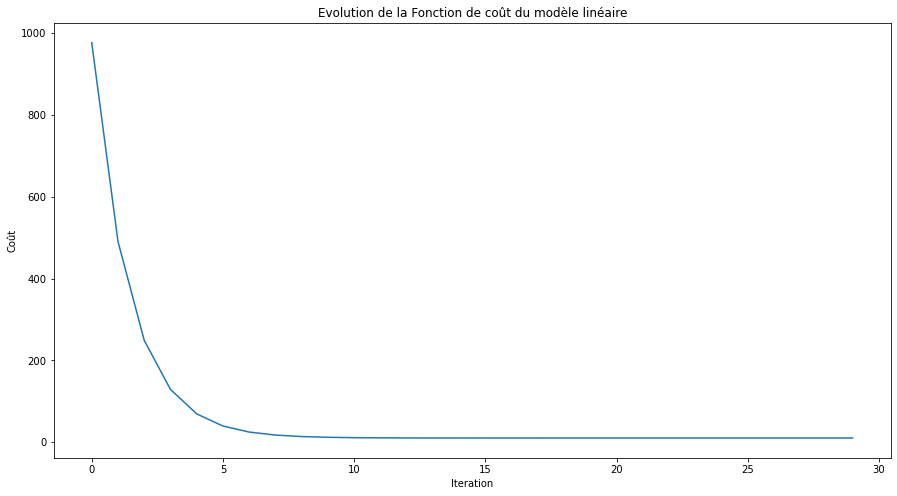
\includegraphics[width=\textwidth]{Rapport/images/cout_MLS.png}
    \caption{Évolution des résultats de la fonctions de coût au fur et à mesure des itérations.}
    \label{fig:JMLS}
\end{figure}

Comme on peut le voir sur ce graphique, notre coût atteint un plateau autour de la 10ème itération, ce qui signifie que notre modèle n'est plus optimisé au-delà. Il aurait donc été possible de ne réaliser que 10 itérations.\\

Il est également possible de représenter l'évolution de notre modèle (voir Fig. \ref{fig:evo_MLS}), grâce à notre varible \textit{F\_plot}. Ce qui nous permet de voir l'amélioration de notre modèle au fur et à mesure des itérations.\\

\begin{figure}[!htbp]
    \centering
    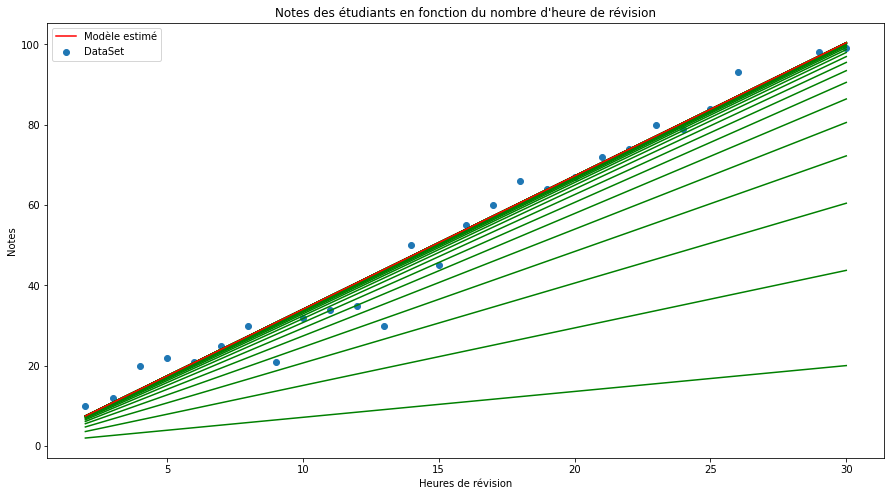
\includegraphics[width=\textwidth]{Rapport/images/evo_MLS.png}
    \caption{Représentation de l'évolution du modèle au fur et à mesure des itérations.}
    \label{fig:evo_MLS}
\end{figure}

Notre modèle peut être évalué par le coefficient de détermination, pour ce faire on utilise la fonction \textit{coeff\_determination}. Pour ce premier modèle notre résultat $R^{2}$ est de \textbf{0.97}, ce qui est un très bon score car on se rapproche de 1.

\subsection{Modèle multiple}

Nous pouvons également utilisé nos fonctions dans le but d'estimer un modèle multiple. Pour ce faire le DataSet \textit{boston\_house\_price.csv} est utilisé. Dans un premier temps on sélectionne les deux variables descriptive les plus corrélées avec notre target. les deux variables sélectionnées sont \textit{LSTAT} et \textit{RM} (voir Fig. \ref{fig:boston_data}).\\

\begin{figure}[!htbp]
    \centering
    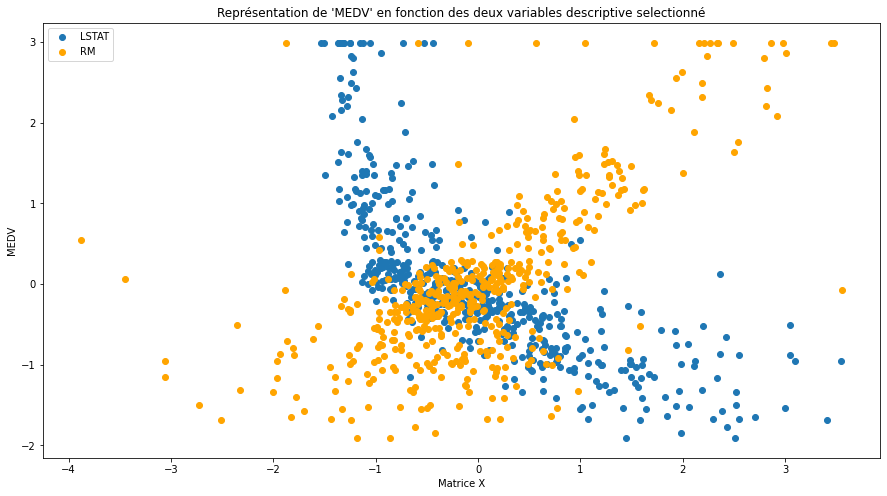
\includegraphics[width=\textwidth]{Rapport/images/data_MLM.png}
    \caption{Représentation de notre target en fonction des deux variables sélectionnés \textit{LSTAT} et \textit{RM}}
    \label{fig:boston_data}
\end{figure}

\noindent Tout comme précédemment on prépare nos matrices et on utilise les fonctions implémentés, on trace ensuite notre graphique de fonction de coût (voir Fig. \ref{fig:cout_MLM}), en adaptant cette fois-ci nos paramètres \textit{alpha} et \textit{n\_iteration}.\\

\begin{figure}[!htbp]
    \centering
    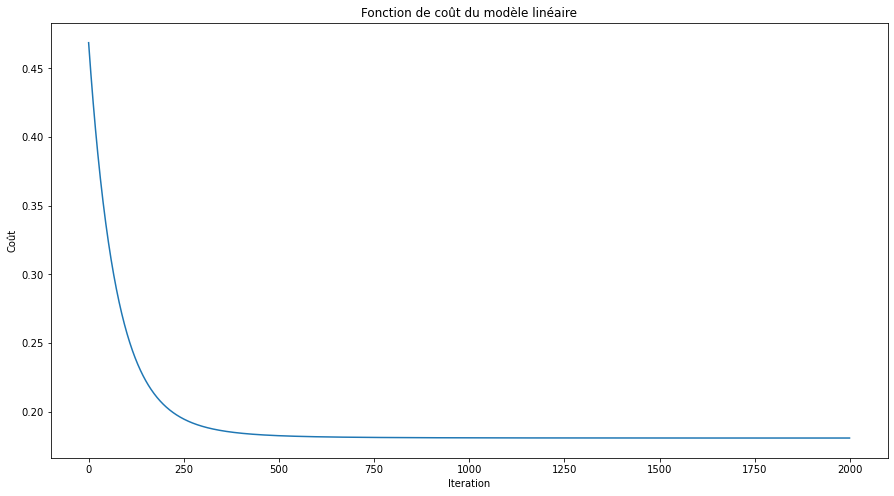
\includegraphics[width=\textwidth]{Rapport/images/cout_MLM.png}
    \caption{Représentation de l'évolution des résultats de la fonctions de coût au fur et à mesure des itérations}
    \label{fig:cout_MLM}
\end{figure}

\noindent Il est possible de constater par cette représentation que nous avons commencer à atteindre un plateau autour de la 1000ème itération. Après évaluation de notre modèle avec le coefficient de détermination on obtient un $R^{2}$ est de \textbf{0.64}. Au vu de ce résultat, on peut envisager que notre modèle n'est pas très bien adapter à ce jeu de données.

\subsection{Modèle polynomiale}

\subsubsection{Jeu de données salaire}

Pour un modèle polynomiale nous pouvons également utilisé nos fonctions. Ici le DataSet utilisé est \textit{Position\_Salaries.csv}. Comme pour les utilisations précédentes on prépare nos matrices, et l'on adapte nos paramètres \textit{alpha} et \textit{n\_iteration}. On représente ensuite la fonction de coût (voir Fig. \ref{fig:cout_MLP}).\\

\begin{figure}[!htbp]
    \centering
    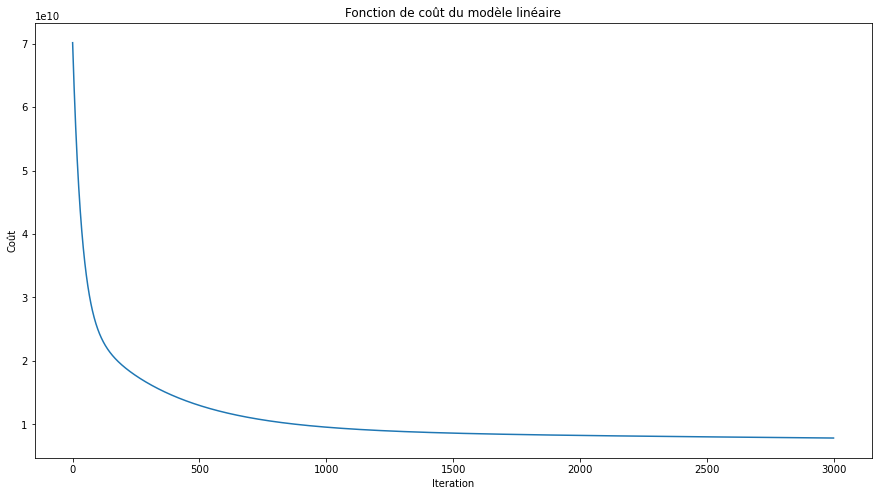
\includegraphics[width=\textwidth]{Rapport/images/cout_MLP.png}
    \caption{Représentation de l'évolution des résultats de la fonctions de coût au fur et à mesure des itérations.}
    \label{fig:cout_MLP}
\end{figure}

Pour ce DataSet on constate que l'on commence à atteindre un plateau autour de la 1500ème itération. Nous avons également tracer l'évolution du modèle en représentant les modèles obtenues toutes les 500 itérations (voir Fig. \ref{fig:evo_MLP}). L'évaluation du modèle avec le coefficient de détermination nous a donné un $R^{2}$ est de \textbf{0.81}. On peut considérer que notre modèle n'est pas le plus optimal, mais son résultat n'est pas non plus mauvais.

\begin{figure}[!htbp]
    \centering
    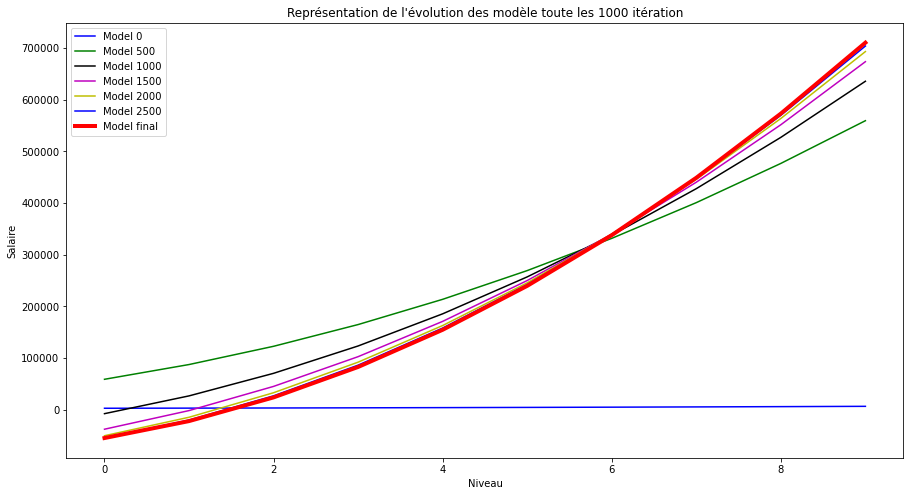
\includegraphics[width=\textwidth]{Rapport/images/evo_MLP.png}
    \caption{Représentation de l'évolution du modèle toutes les 500 itérations.}
    \label{fig:evo_MLP}
\end{figure}

\subsubsection{Jeu de données vin}

On réalise les mêmes étapes que les précédentes sur le jeu de données \textit{qualite-vin-rouge.csv}. On réalise une corrélation pour identifier la variable déscriptive la plus corrélé avec notre target (\textit{"qualité"}). On établis nos différentes matrices, et on lance l'estimation de notre modèle. Il est possible de constater sur la courbe de fonction coût (voir Fig. \ref{fig:cout_MLP2}), qu'un plateau est atteint autour de la 500ème itération.\\

\begin{figure}[!htbp]
    \centering
    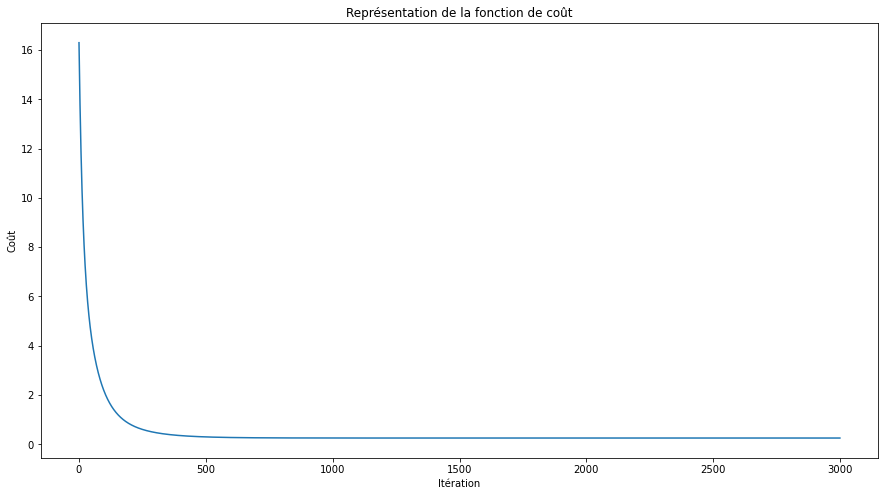
\includegraphics[width=\textwidth]{Rapport/images/cout_MLP2.png}
    \caption{Représentation de l'évolution des résultats de la fonctions de coût au fur et à mesure des itérations.}
    \label{fig:cout_MLP2}
\end{figure}

\noindent Pour l'évaluation de modèle on a eu pour le coefficient de détermination \textbf{0.23}, et pour l'erreur quadratique moyenne \textbf{0.5}. Au vu de ces valeurs notre modèle n'est pas fiable.\\

\noindent En représentant notre modèle sur les données (voir Fig. \ref{fig:modele_mlp2}),on constate que notre jeu de données correspond à de la catégorisation. Notre approche n'est donc pas approprié à ce type de données, il faudrait peut-être réfléchir à une autre méthode.

\begin{figure}[!htbp]
    \centering
    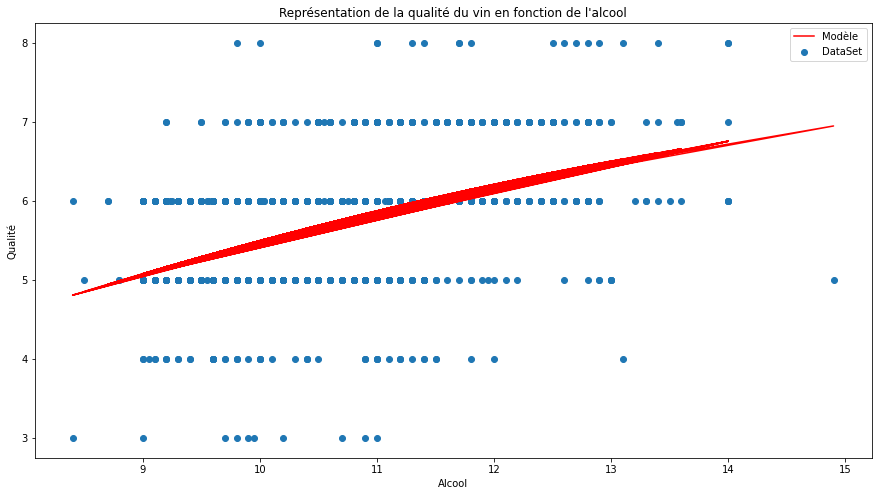
\includegraphics[width=\textwidth]{Rapport/images/modele_MLP2.png}
    \caption{Représentation du modèle estimé.}
    \label{fig:modele_mlp2}
\end{figure}

\newpage

\section{Comparaison des résultats}

\subsection{Modèle simple}

\begin{figure}[!htbp]
    \centering
    \begin{subfigure}[b]{0.49\textwidth}
         \centering
         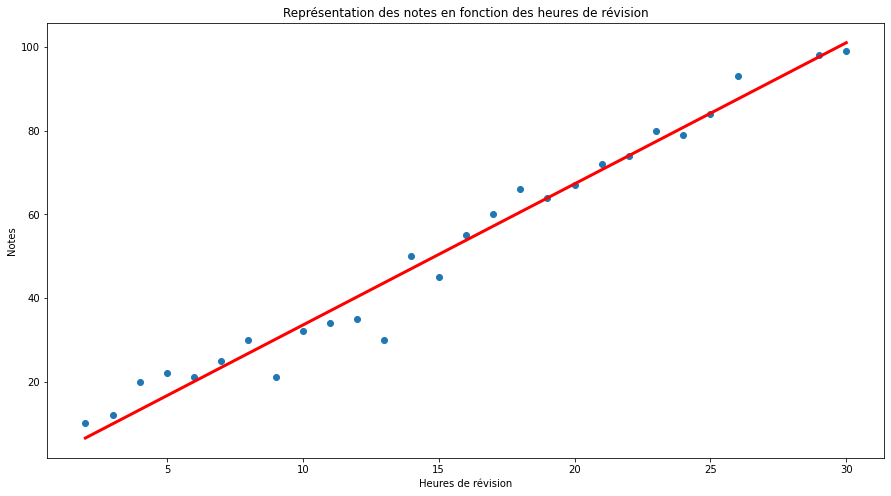
\includegraphics[width=\textwidth]{Rapport/images/modele_LS.png}
         \caption{Fonction implémentée}
        \label{fig:modele_LS}
    \end{subfigure}
    \begin{subfigure}[b]{0.5\textwidth}
         \centering
         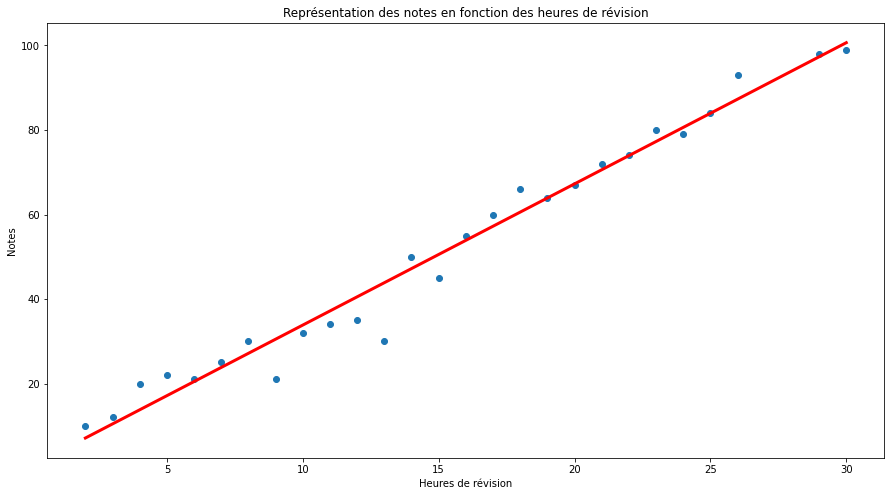
\includegraphics[width=\textwidth]{Rapport/images/modele_SLLS.png}
         \caption{ScikitLearn}
        \label{fig:modele_SLLS}
    \end{subfigure}
    \caption{Comparaison des modèles obtenu par la fonction de régression Linéaire implémenter manuellement (a) et celle de de ScikitLearn (b)}
\end{figure}


\subsection{Modèle polynomiale - \textit{Position\_Salaries.csv}}

\begin{figure}[!htbp]
    \centering
    \begin{subfigure}[b]{0.49\textwidth}
         \centering
         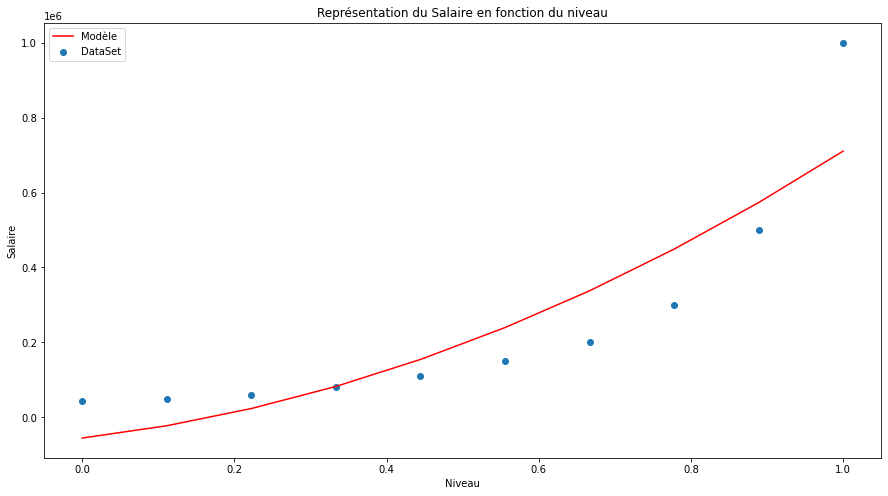
\includegraphics[width=\textwidth]{Rapport/images/modele_MLP.png}
         \caption{Fonction implémentée}
        \label{fig:modele_LP1}
    \end{subfigure}
    \begin{subfigure}[b]{0.5\textwidth}
         \centering
         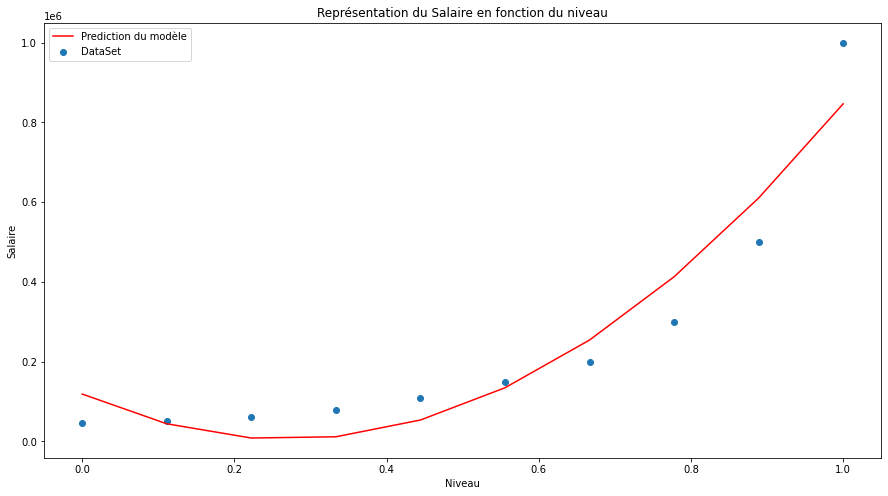
\includegraphics[width=\textwidth]{Rapport/images/modele_SLLP1.png}
         \caption{ScikitLearn}
        \label{fig:modele_SLLP1}
    \end{subfigure}
    \caption{Comparaison des modèles obtenu par la fonction de régression Linéaire implémenter manuellement (a) et celle de de ScikitLearn (b)}
\end{figure}

\subsection{Modèle polynomiale - \textit{qualite-vin-rouge.csv}}

\begin{figure}[!htbp]
    \centering
    \begin{subfigure}[b]{0.49\textwidth}
         \centering
         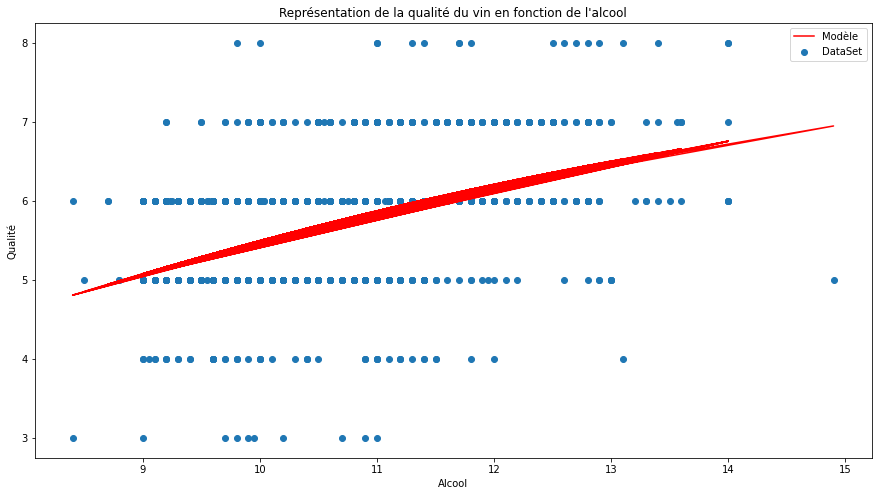
\includegraphics[width=\textwidth]{Rapport/images/modele_MLP2.png}
         \caption{Fonction implémentée}
        \label{fig:modele_LP1}
    \end{subfigure}
    \begin{subfigure}[b]{0.5\textwidth}
         \centering
         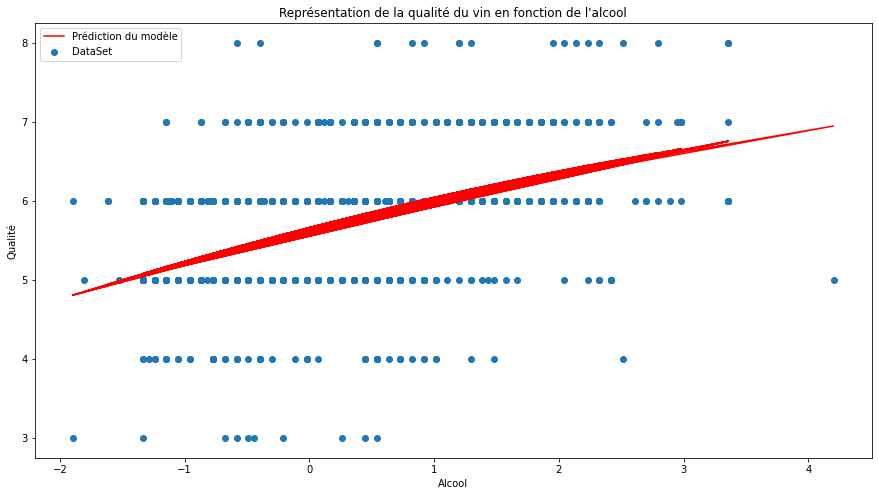
\includegraphics[width=\textwidth]{Rapport/images/modele_SLP2.png}
         \caption{ScikitLearn}
        \label{fig:modele_SLLP1}
    \end{subfigure}
    \caption{Comparaison des modèles obtenu par la fonction de régression Linéaire implémenter manuellement (a) et celle de de ScikitLearn (b)}
\end{figure}

\newpage

\subsection{Récapitulatif des évaluations des modèles}

Le tableau ci-dessous regroupe les résultats obtenus lors des évaluations des différents modèles avec le coefficient de détermination et l'erreur quadratique moyenne. Les valeurs obtenus nous montre qu'il n'y a que très peu de différence entre l'utilisation des fonctions de Scikit Learn et celles que nous avons implémenté manuellement. Sauf pour le modèle polynomiale basé sur le DataSet \textit{Position\_Salaries.csv}, où l'on observe un meilleur $R^{2}$ pour la fonction de Scikit Learn. Cela pourrait peut-être s'expliquer par le fait que les paramètres utilisé dans notre fonction ne correspondait pas à ceux utilisé par défaut dans Scikit Learn.\\

\begin{table}[!htbp]
\begin{tabular}{l|cc|cc|}
\cline{2-5}
                                                        & \multicolumn{2}{l|}{\textbf{Fonction manuelles}}     & \multicolumn{2}{l|}{\textbf{Fonction Scikit Learn}}  \\ \cline{2-5} 
                                                        & \multicolumn{1}{c|}{\textbf{$R^{2}$}} & \textbf{MSE} & \multicolumn{1}{c|}{\textbf{$R^{2}$}} & \textbf{MSE} \\ \hline
\multicolumn{1}{|l|}{\textbf{Modèle linéaire simple}}   & \multicolumn{1}{c|}{0.97}             & -            & \multicolumn{1}{c|}{0.97}             & -            \\ \hline
\multicolumn{1}{|l|}{\textbf{Modèle linéaire multiple}} & \multicolumn{1}{c|}{0.64}             & 0.36         & \multicolumn{1}{c|}{0.64}             & 0.36         \\ \hline
\multicolumn{1}{|l|}{\textbf{Modèle polynomiale 1}}     & \multicolumn{1}{c|}{0.81}             & $1.6e^{10}$  & \multicolumn{1}{c|}{0.92}             & $6.8e^{9}$   \\ \hline
\multicolumn{1}{|l|}{\textbf{Modèle polynomiale 2}}     & \multicolumn{1}{c|}{0.23}             & 0.50         & \multicolumn{1}{c|}{0.23}             & 0.50         \\ \hline
\end{tabular}
\caption{Tableau de comparaison des valeurs de $R^{2}$ et de MSE obtenue par les modèles estimés par les fonctions implémenter manuellement, et les modèles obtenus par l'utilisation de Scikit Learn}
\label{tab:comparatif}
\end{table}

Pour conclure cette comparaison, on pourrait dire que le fait d'implémenter une fonction soit même nous offre une meilleur maîtrise de son utilisation. Cependant, on peut considérer que les fonctions Scikit Learn ont sûrement était plus optimisé que les nôtres. Avec des résultats aussi similaire autant utiliser les fonctions déjà existantes qui nous permettant même dans certain cas d'obtenir de meilleurs résultats.

\section{Conclusion}

En conclusion ce projet m'a permis de revoir des notions que je connaissais déjà, je n'ai donc rien appris de nouveaux, cependant cela m'a permit de consolider mes connaissances. Aucunes difficultés à signaler.

\end{document}
